\documentclass[a4paper,10pt]{article}
\usepackage[utf8]{inputenc}
\usepackage{amsmath}
\usepackage{graphicx}
\numberwithin{equation}{section}
%opening
\title{Math Phys II HW 2}
\author{Vince Baker}

\begin{document}

\maketitle

\begin{abstract}

\end{abstract}

\section{Problem 1}
We seek solutions of the Kortweg-deVries equation:
\begin{equation}
 \frac{\partial \psi}{\partial t}+\psi\frac{\partial \psi}{\partial x}+\frac{\partial ^3 \psi}{\partial x^3}=0
\end{equation}
We look for solutions $\psi(\xi)$, with $\xi=x-ct$. To write 1.1 in terms of $\xi$, we calculate the partial derivatives:
\begin{gather*}
 \frac{\partial \psi}{\partial t}=-c\frac{d \psi(\xi)}{d \xi}\\
 \frac{\partial \psi}{\partial x}=\frac{d \psi(\xi)}{d \xi}\\
 \frac{\partial^3 \psi}{\partial x^3}=\frac{d^3 \psi(\xi)}{d \xi ^3}
\end{gather*}
We can now write 1.1 in terms of $\xi$:
\begin{equation} 
-c\frac{d \psi}{d \xi}+\psi\frac{d \psi}{d \xi}+\frac{d^3 \psi}{d \xi ^3}=0
\end{equation}
This simplifies to:
\begin{equation}
 (\psi-c)\frac{d \psi}{d \xi}+\frac{d^3 \psi}{d \xi ^3}=0
\end{equation}
We can integrate 1.3 to find:
\begin{equation}
 \frac{d^2\psi}{d\xi^2}=c\psi-\frac{\psi^2}{2}
\end{equation}
We then integrate again and multiply by $\frac{d \psi}{d \xi}$:
\begin{gather}
\frac{d\psi}{d\xi}=\int(c\psi-\frac{\psi^2}{2})\\
(\frac{d\psi}{d\xi})^2=\frac{\psi^2}{2}(c-\frac{\psi}{3})\\
\frac{d\psi}{d\xi}=\frac{\psi}{\sqrt{2}}(c-\frac{\psi}{3})^\frac{1}{2}
\end{gather}
We can now integrate for $\xi$ using Wolfram Alpha:
\begin{equation}
 \xi =\int \frac{d \psi}{\frac{\psi}{\sqrt{2}}(c-\frac{\psi}{3})^{\frac{1}{2}}}
 =\frac{2\sqrt{2}\ tanh^{-1}(\frac{\sqrt{c-\frac{\psi}{3}}}{\sqrt{c}})}{\sqrt{c}}
\end{equation}
And then rearrange to find $\psi$ as a function of $\xi$ and c.
\begin{gather}
 \xi \sqrt{c}=2\sqrt{2}\ tanh^{-1}(\sqrt{1-\frac{\psi}{3c}} )\\
 \frac{\xi \sqrt{c}}{2\sqrt{2}}=tanh^{-1}(\sqrt{1-\frac{\psi}{3c}} )\\
 tanh(\frac{\xi \sqrt{c}}{2\sqrt{2}})=\sqrt{1-\frac{\psi}{3c}}\\
 tanh^{2}(\frac{\xi \sqrt{c}}{2\sqrt{2}})=1-\frac{\psi}{3c}\\
 \psi=3c\{1-tanh^{2}(\frac{\xi \sqrt{c}}{2\sqrt{2}})\}\\
 \psi=\frac{3c}{cosh^{2}(\frac{\xi}{2}\sqrt{\frac{c}{2}})}
\end{gather}

\section{Problem 2}
The general form of a second-order linear PDE is:
\begin{equation}
 A(x,y)\frac{\partial ^2 \psi}{\partial x^2}+2B(x,y)\frac{\partial ^2\psi}{\partial x \partial y}+C(x,y)\frac{\partial ^2 \psi}{\partial y^2}
\end{equation}
The characteristic equation,  with solutions $\xi(x,y)$ and $\eta(x,y)$, is:
\begin{equation}
 A(\frac{dy}{dx})^2+2B(\frac{dy}{dx})+C=0
\end{equation}
We wish to write Eq. 1 in terms of $\xi$ and $\eta$. We differentiate $\psi(\xi, \eta)$:
\begin{gather}
\frac{\partial \psi}{\partial x}=\frac{\partial \psi}{\partial \xi}\frac{\partial \xi}{\partial x}+\frac{\partial \psi}{\partial \eta}\frac{\partial \eta}{\partial x}
\end{gather}
Now we calculate the other partials with respect to $\eta$ and $\xi$.
\begin{gather}
\frac{\partial}{\partial x}(\frac{\partial \psi}{\partial \xi})=\frac{\partial ^2 \psi}{\partial \xi^2}\frac{\partial \xi}{\partial x}+
\frac{\partial ^2 \psi}{\partial \xi \partial \eta}\frac{\partial \eta}{\partial x}\\
\frac{\partial}{\partial x}(\frac{\partial \psi}{\partial \eta})=\frac{\partial ^2 \psi}{\partial \eta^2}\frac{\partial \eta}{\partial x}+
\frac{\partial ^2 \psi}{\partial \xi \partial \eta}\frac{\partial \xi}{\partial x}
\end{gather}
We use 3,4 and 5 to calculate $\frac{\partial ^2 \psi}{\partial x^2}$.
\begin{gather*}
\frac{\partial ^2 \psi}{\partial x^2} = \frac{\partial ^2 \xi}{\partial x^2}\frac{\partial \psi}{\partial \xi}
+\frac{\partial \xi}{\partial x}(\frac{\partial ^2 \psi}{\partial \xi^2}\frac{\partial \xi}{\partial x}+
\frac{\partial ^2 \psi}{\partial \xi \partial \eta}\frac{\partial \eta}{\partial x})\\
+\frac{\partial ^2 \eta}{\partial x^2}\frac{\partial \psi}{\partial \eta}
+\frac{\partial \eta}{\partial x}(\frac{\partial ^2 \psi}{\partial \eta^2}\frac{\partial \eta}{\partial x}+
\frac{\partial ^2 \psi}{\partial \xi \partial \eta}\frac{\partial \xi}{\partial x})\\
=\frac{\partial ^2 \xi}{\partial x^2}\frac{\partial \psi}{\partial \xi}+\frac{\partial ^2 \eta}{\partial x^2}\frac{\partial \psi}{\partial \eta}
+\frac{\partial ^2 \psi}{\partial \xi ^2}(\frac{\partial \xi}{\partial x})^2 +\frac{\partial \xi}{\partial x}\frac{\partial \eta}{\partial x}
\frac{\partial ^2 \psi}{\partial \xi \partial \eta}+\frac{\partial ^2 \psi}{\partial \eta ^2}(\frac{\partial \eta}{\partial x})^2
+\frac{\partial \xi}{\partial x}\frac{\partial \eta}{\partial x}\frac{\partial ^2 \psi}{\partial \xi \partial \eta}
\end{gather*}
\begin{gather}
\frac{\partial ^2 \psi}{\partial x^2}=\frac{\partial ^2 \xi}{\partial x^2}\frac{\partial \psi}{\partial \xi}+\frac{\partial ^2 \eta}{\partial x^2}
\frac{\partial \psi}{\partial \eta}
+\frac{\partial ^2 \psi}{\partial \xi ^2}(\frac{\partial \xi}{\partial x})^2+\frac{\partial ^2 \psi}{\partial \eta ^2}(\frac{\partial \eta}{\partial x})^2
+2(\frac{\partial \xi}{\partial x}\frac{\partial \eta}{\partial x}\frac{\partial ^2 \psi}{\partial \xi \partial \eta})
\end{gather}
The calculation of $\frac{\partial ^2 \psi }{\partial y^2}$ is identical.
\begin{gather}
\frac{\partial ^2 \psi}{\partial y^2}=\frac{\partial ^2 \xi}{\partial y^2}\frac{\partial \psi}{\partial \xi}+\frac{\partial ^2 \eta}{\partial y^2}\frac{\partial \psi}{\partial \eta}
+\frac{\partial ^2 \psi}{\partial \xi ^2}(\frac{\partial \xi}{\partial y})^2+\frac{\partial ^2 \psi}{\partial \eta ^2}(\frac{\partial \eta}{\partial y})^2
+2(\frac{\partial \xi}{\partial y}\frac{\partial \eta}{\partial y}\frac{\partial ^2 \psi}{\partial \xi \partial \eta})
\end{gather}
We now take $\frac{\partial}{\partial y}$ of equation 1:
\begin{multline}
 \frac{\partial ^2\psi}{\partial x \partial y}=\frac{\partial ^2\xi}{\partial x \partial y}\frac{\partial \psi}{\partial \xi}
 +\frac{\partial ^2 \eta}{\partial x \partial y}\frac{\partial \psi}{\partial \eta}
 +\frac{\partial^2 \psi}{\partial \xi ^2}(\frac{\partial \xi}{\partial x}\frac{\partial \xi}{\partial y})\\
 +\frac{\partial^2 \psi}{\partial \eta ^2}(\frac{\partial \eta}{\partial x}\frac{\partial \eta}{\partial y})
 +\frac{\partial ^2 \psi}{\partial \xi \partial \eta}(\frac{\partial \xi}{\partial x}\frac{\partial \eta}{\partial y}+\frac{\partial \eta}{\partial x}\frac{\partial \xi}{\partial y} ) 
\end{multline}

We can now write Eq. 1 in terms of $\xi$ and $\eta$:
\begin{multline}
 A\{\frac{\partial ^2 \xi}{\partial x^2}\frac{\partial \psi}{\partial \xi}+\frac{\partial ^2 \eta}{\partial x^2}
\frac{\partial \psi}{\partial \eta}
+\frac{\partial ^2 \psi}{\partial \xi ^2}(\frac{\partial \xi}{\partial x})^2+\frac{\partial ^2 \psi}{\partial \eta ^2}(\frac{\partial \eta}{\partial x})^2
+2(\frac{\partial \xi}{\partial x}\frac{\partial \eta}{\partial x}\frac{\partial ^2 \psi}{\partial \xi \partial \eta})\}\\
+2B\{\frac{\partial ^2\xi}{\partial x \partial y}\frac{\partial \psi}{\partial \xi}
 +\frac{\partial ^2 \eta}{\partial x \partial y}\frac{\partial \psi}{\partial \eta}
 +\frac{\partial^2 \psi}{\partial \xi ^2}(\frac{\partial \xi}{\partial x}\frac{\partial \xi}{\partial y})\\
 +\frac{\partial^2 \psi}{\partial \eta ^2}(\frac{\partial \eta}{\partial x}\frac{\partial \eta}{\partial y})
 +\frac{\partial ^2 \psi}{\partial \xi \partial \eta}(\frac{\partial \xi}{\partial x}\frac{\partial \eta}{\partial y}+\frac{\partial \eta}{\partial x}\frac{\partial \xi}{\partial y} ) \}\\
 +C\{\frac{\partial ^2 \xi}{\partial y^2}\frac{\partial \psi}{\partial \xi}+\frac{\partial ^2 \eta}{\partial y^2}\frac{\partial \psi}{\partial \eta}
+\frac{\partial ^2 \psi}{\partial \xi ^2}(\frac{\partial \xi}{\partial y})^2+\frac{\partial ^2 \psi}{\partial \eta ^2}(\frac{\partial \eta}{\partial y})^2
+2(\frac{\partial \xi}{\partial y}\frac{\partial \eta}{\partial y}\frac{\partial ^2 \psi}{\partial \xi \partial \eta}) \}=0
\end{multline}
We now take a break to stop Eq. 9 from giving us a migraine brought on by eye strain.

We collect the coefficients of all the derivates of $\psi$:
\begin{gather}
\frac{\partial \psi}{\partial \xi}(A\frac{\partial ^2 \xi}{\partial x^2}+2B\frac{\partial ^2 \xi}{\partial x \partial y}+C\frac{\partial ^2 \xi}{\partial y^2})\\
\frac{\partial \psi}{\partial \eta}(A\frac{\partial ^2 \eta}{\partial x^2}+2B\frac{\partial ^2 \eta}{\partial x \partial y}+C\frac{\partial ^2 \eta}{\partial y^2})\\
\frac{\partial ^2 \psi}{\partial \xi ^2}(A(\frac{\partial \xi}{\partial x})^2+2B\frac{\partial \xi}{\partial x}\frac{\partial \xi}{\partial y}+C(\frac{\partial \xi}{\partial y})^2)\\
\frac{\partial ^2 \psi}{\partial \eta ^2}(A(\frac{\partial \eta}{\partial x})^2+2B\frac{\partial \eta}{\partial x}\frac{\partial \eta}{\partial y}+C(\frac{\partial \eta}{\partial y})^2)\\
\frac{\partial ^2 \psi}{\partial \xi \partial \eta}(2A(\frac{\partial \xi}{\partial x}\frac{\partial \eta}{\partial x})
+2B(\frac{\partial \xi}{\partial x}\frac{\partial \eta}{\partial y}+\frac{\partial \xi}{\partial y}\frac{\partial \eta}{\partial x})
+2C(\frac{\partial \xi}{\partial y}\frac{\partial \eta}{\partial y}))
\end{gather}
We recognize that since $\xi(x,y)$ and $\eta(x,y)$ are solutions to Eq. 2.2, along a characteristic curve:
\begin{gather}
 \xi (x,y) = constant\\
 \frac{dy}{dx}=\frac{\partial \xi}{\partial x} (-\frac{\partial \xi}{\partial y})^{-1}\\
  A(\frac{\partial \xi}{\partial x} (-\frac{\partial \xi}{\partial y})^{-1})^2
 +2B(\frac{\partial \xi}{\partial x} (-\frac{\partial \xi}{\partial y})^{-1})
 +C=0\\
 A(\frac{\partial \xi}{\partial x})^2+2B\frac{\partial \xi}{\partial x}\frac{\partial \xi}{ \partial y}+C(\frac{\partial \xi}{\partial y})^2=0\\
\end{gather}
The same argument also implies:
\begin{equation}
  A(\frac{\partial \eta}{\partial x})^2+2B\frac{\partial \eta}{\partial x}\frac{\partial \eta}{ \partial y}+C(\frac{\partial \eta}{\partial y})^2=0
\end{equation}
So 2.12 and 2.13 are both equal to 0 and we've removed most second derivates of $\psi$. 
We now collect the $\frac{\partial ^2}{\partial \xi \partial \eta}$ on the left and everything else on the right.
\begin{multline}
\frac{\partial ^2 \psi}{\partial \xi \partial \eta}(2A(\frac{\partial \xi}{\partial x}\frac{\partial \eta}{\partial x})
+2B(\frac{\partial \xi}{\partial x}\frac{\partial \eta}{\partial y}+\frac{\partial \xi}{\partial y}\frac{\partial \eta}{\partial x})
+2C(\frac{\partial \xi}{\partial y}\frac{\partial \eta}{\partial y}))=\\
\frac{\partial \psi}{\partial \xi}(A\frac{\partial ^2 \xi}{\partial x^2}+2B\frac{\partial ^2 \xi}{\partial x \partial y}+C\frac{\partial ^2 \xi}{\partial y^2})+
\frac{\partial \psi}{\partial \eta}(A\frac{\partial ^2 \eta}{\partial x^2}+2B\frac{\partial ^2 \eta}{\partial x \partial y}+C\frac{\partial ^2 \eta}{\partial y^2})
\end{multline}
Dividing the awful mess on the right side by the slightly-less-awful mess on the left:
\begin{multline}
\frac{\partial ^2 \psi}{\partial \xi \partial \eta}=\\
\frac{\frac{\partial \psi}{\partial \xi}(A\frac{\partial ^2 \xi}{\partial x^2}+2B\frac{\partial ^2 \xi}{\partial x \partial y}+C\frac{\partial ^2 \xi}{\partial y^2})+
\frac{\partial \psi}{\partial \eta}(A\frac{\partial ^2 \eta}{\partial x^2}+2B\frac{\partial ^2 \eta}{\partial x \partial y}+C\frac{\partial ^2 \eta}{\partial y^2})}
{2(A(\frac{\partial \xi}{\partial x}\frac{\partial \eta}{\partial x})
+B(\frac{\partial \xi}{\partial x}\frac{\partial \eta}{\partial y}+\frac{\partial \xi}{\partial y}\frac{\partial \eta}{\partial x})
+C(\frac{\partial \xi}{\partial y}\frac{\partial \eta}{\partial y}))}
\end{multline}
The right-hand side depends only on first derivates of $\psi$, the known functions A/B/C, and known derivatives of $\xi$ and $\eta$.

\section{Problem 3}
We are solving the characteristic equation for:
\begin{gather*}
 \frac{\partial ^2\psi}{\partial t^2}-c(x)^2\frac{\partial ^2 \psi}{\partial x^2}=0\\
\end{gather*}
With A=1, B=0, and $c=-c(x)^2$, the characteristic equation is:
\begin{gather}
(\frac{dx}{dt})^2-c(x)^2=0\\
\frac{dx}{dt}=\pm c(x)\\
dt=\pm\frac{1}{c(x)}dx
\end{gather}
With $c(x)=c_0(1+\frac{|x|}{a})$ the characteristic curve can be written:
\begin{equation}
t=\pm\frac{1}{c_0}(x+sgn(x)\frac{x^2}{2a})+C
\end{equation}
Several characteristic curves are shown below for a-values 0.01, 0.1, 1, 10 and $10^{6}$. 
The positive curves are shown in blue, the negative curves in red.
The large value of a produces nearly straight lines.

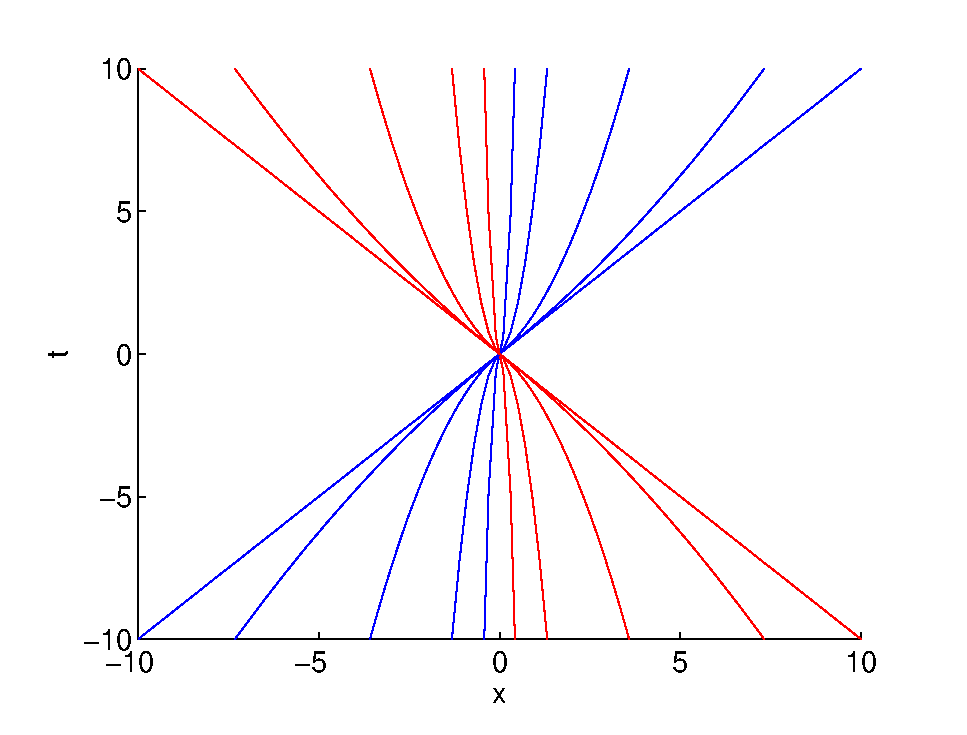
\includegraphics{p3chars}

We now look to find a solution given the initial conditions:
\begin{gather}
\psi(x,0)=0\\
\frac{\partial \psi}{\partial t}\mid_{t=0}=e^{-|x|}
\end{gather}
When $a=\infty$ the characteristic solutions become:
\begin{gather}
\xi=x+c_0t\\
\eta=x-c_0t
\end{gather}
These characteristic curves are consistent with the large value of a plotted above.
The solution can be written as a combination $\psi=f(\xi)+g(\eta)$. 
Using the initial condition $\psi(x,0)=0$ we see that $f(x)+g(x)=0$, so that $g(x)=-f(x)$.
We also note that, since $x>0$, $e^{-|x|}=e^{-x}$.
We differentiate the combined solution with respect to t and use the second boundary condition:
\begin{gather}
-v\frac{df}{dt}+c_0\frac{dg}{dt}=e^{-x}\\
\int-2\frac{df}{dt}=\int\frac{1}{c_0}e^{-x}\\
f=\frac{-1}{2c_0}e^{-x}
\end{gather}
We can now write the combined solution:
\begin{equation}
\psi(x,t)=\frac{1}{2c_0}(e^{-x+vt}-e^{-x-vt}) 
\end{equation}

\section{Problem 4}
We solve the diffusion equation for the temperature in a uniform cube of side L.

\begin{equation}
 \nabla^2T=\frac{1}{\kappa}\frac{\partial T}{\partial t}
\end{equation}
We first separate T into time and space terms.
\begin{gather}
 T=\Gamma (t)\Psi(\vec{r})\\
 \nabla ^2T=\nabla ^2 \Psi \Gamma\\
 \frac{\partial T}{\partial t}=\Psi \Gamma ^{\prime}\\
 \frac{\nabla ^2 \Psi}{\Psi}-\frac{1}{\kappa}\frac{\Gamma ^{\prime}}{\Gamma}=0\\
 \frac{\nabla ^2 \Psi}{\Psi}=-\frac{1}{\kappa}\frac{\Gamma ^{\prime}}{\Gamma}=v^2\\
\end{gather}
We can now solve the time dependent part.
\begin{gather}
\Gamma ^{\prime}=\Gamma kv^2\\
\Gamma ^{\prime}-kv^2\Gamma=0\\
\Gamma=\alpha e^{-tkv^2}
\end{gather}
The boundary condition $\Gamma=0$ at $t=0$ can't be satisfied by this equation, so we shift the temperature scale so that the system
starts at $T=-T_0$ and the heat bath is at a temperature of 0. We can then solve for $\alpha$.
\begin{gather}
\alpha = -T_0\\
\Gamma=-T_0 e^{-tkv^2}
\end{gather}

We now separate the X/Y/Z components of the spatial function.
\begin{gather}
\Psi (\vec{r})=X(x)Y(y)Z(z)\\
\frac{\nabla ^2\Psi}{\Psi}=v^2\\
\nabla ^2\Psi -v^2 \Psi =0\\
X^{''} YZ+XY^{''} Z+XYZ^{''} +v^2XYZ=0\\
\frac{X^{''} }{X}+\frac{Y^{''} }{Y}+\frac{Z^{''} }{Z}-v^2=0\\
X^{''} +a^2 X=0\\
Y^{''} +b^2 Y=0\\
Z^{''} +c^2 Z=0\\
a^2+b^2+c^2=v^2
\end{gather}
The spatial functions are all zero at both 0 and L (since we've shifted the temperature scale so the heat bath is at 0).
The solutions are:
\begin{gather}
X=sin\frac{\ell \pi}{L}x\\
Y=sin\frac{m\pi}{L}y\\
Z=sin\frac{n \pi}{L}z\\
a=\frac{\ell L}{\pi},\ b=\frac{mL}{\pi},\ \gamma=\frac{nL}{\pi}
\end{gather}
We can now write the general solution to the equation as a linear combination of the separate solutions.
\begin{equation}
T=\sum _{\ell,m,n=0}^{\infty}v^2_{\ell mn}(-T_0)e^{-tkv_{\ell mn}^{2}}\ sin(\frac{\ell \pi}{L}x)\ sin(\frac{m \pi}{L}y)\ sin(\frac{n \pi}{L}z)
\end{equation}
With $\ell, m, n$ integers and subject to $\frac{\pi^2}{L^2}(\ell^2+m^2+n^2)=v^2$. 
We can use the boundary condition at t=0 to find $v^2_{\ell mn}$. 
Since the XYZ terms are all sines we use the tyical method for finding coefficients of a Fourier series.
\begin{gather}
 v^2_{\ell mn}=(\frac{2}{L})^3 \int_0^L \int_0^L \int_0^L dx\ dy\ dz\ -T_0sin(\frac{\ell \pi}{L}x)\ sin(\frac{m\pi}{L}y)\ sin(\frac{n \pi}{L}z)\\ 
 v^2_{\ell mn}=\frac{-T_08}{L^2 \pi}\{\frac{1}{\ell}(1-(-1)^\ell )\ \frac{1}{m}(1-(-1)^m )\ \frac{1}{n}(1-(-1)^n) \} 
\end{gather}


\section{Problem 5}
We solve the wave equation for a particle confined to a cylinder of radius $R_0$ and height H.
\begin{gather}
\frac{-\hbar ^2}{2m} \nabla ^2 \psi=E \psi\\
\nabla ^2 \psi +k^2\psi=0, k\equiv \sqrt{\frac{2mE}{\hbar ^2}}
\end{gather}
We separate the equation into functions in cylindrical coordinates.
\begin{gather}
 \psi=R(r)\Phi(\phi)Z(z)\\
 \frac{1}{r}\frac{\partial}{\partial r}(r\frac{dR}{dr})\Phi Z+\frac{1}{r^2}\frac{d \Phi ^2}{d \phi }RZ+\frac{d^2Z}{dz}R\Phi +k^2r\Phi Z=0\\
 \frac{1}{rR}\frac{d}{dr}(rR^{'} )+\frac{1}{r^2}\frac{\Phi^{''} }{\Phi}+\frac{Z^{''}}{Z}+k^2=0
\end{gather}
We can now solve for Z incorporating the boundary conditions that $\psi=0$ at z=0,H.
\begin{gather}
\frac{Z^{''}}{Z}=const.=a^2\\
 Z^{''}-a^2Z=0\\
 Z=sin\frac{\ell \pi}{H}z,\ a^2=(\frac{\ell \pi}{H})^2
\end{gather}
Substituing the constant value of $\frac{Z^{''}}{Z}$ into 5.5 and multiplying by $r^2$, we get:
\begin{equation}
\frac{r}{R}\frac{d}{dr}(rR^{'})+\frac{\Phi ^{''}}{\Phi}+r^2(a^2+k^2)=0 
\end{equation}
we can now separate the $\Phi$ term.
\begin{gather}
\frac{\Phi ^{''}}{\Phi}=const.=-m^2\\
\Phi ^{''}+m^2\Phi=0
\end{gather}
There is no explicit boundary condition on $\phi$. 
However, since $\phi$ is an angular coordinate $\Phi$ must be single-valued on multiples of $2\pi$. 
With $\Phi(0)=\Phi(2\pi)$, the solution is a general exponential with m confined to integer values.
\begin{equation}
\Phi=e^{im \phi}, \  m=0,1,2...
\end{equation}
Using the constant value of $\frac{\Phi ^{''}}{\Phi } $ in 5.7, we now solve the radial part.
\begin{gather}
 \frac{r}{R}\frac{d}{dr}(rR^{'})+\frac{\Phi ^{''}}{\Phi}+r^2(a^2+k^2)=0 \\
 \frac{r}{R}\frac{d}{dr}(rR^{'})-m^2+r^2n^2=0,\  n^2\equiv a^2+k^2\\ 
 \frac{r}{R}(R^{'}+rR{''})-m^2+r^2n^2=0\\ 
 r^2R^{''}+rR^{'}+R(r^2n^2-m^2)=0
\end{gather}
This is not quite the right form for Bessel's equation, so we make the substitution $x=nr$.
\begin{gather}
 x=nr\\
 x\frac{dR}{dx}=nr\frac{1}{n}\frac{dR}{dr}=r\frac{dR}{dr}\\
 x^2\frac{d^2R}{dx^2}=(nr)^2(\frac{1}{n})^2\frac{d^2R}{dr^2}=r^2\frac{d^2R}{dr^2}\\
 x^2R^{''}+xR^{'}+R(x^2-m^2)=0
\end{gather}
The solutions are Bessel's functions $J_{m}(x)=J_{m}(nr)$. 
The boundary condition $\Psi=0$ at $R_0$ restricts the values of n to $\frac{\alpha_{ms}}{R_0}$, with $\alpha_{ms}$ the $s^{th}$ root of $J_{m}$. 
The energy levels can be found from eq. 5.2:
\begin{gather}
 n=\frac{\alpha_{ms}}{R_0}\\
 k^2=\frac{2mE}{\hbar ^2}=n^2+a^2=(\frac{\alpha_{ms}}{R_0})^2+(\frac{\ell \pi}{H})^2\\
 E=\frac{\hbar^2}{2m}\{(\frac{\alpha_{ms}}{R_0})^2+(\frac{\ell \pi}{H})^2 \}
\end{gather}
The minimum energy level is $\alpha_{01}=2.4048,\ \ell=1$. The minimum energy is therefore:
\begin{equation}
  E_0=\frac{\hbar^2}{2m}\{(\frac{2.4048}{R_0})^2+(\frac{\pi}{H})^2 \}
\end{equation}
In the ground state m=0 so the $\phi$ term is 1. The ground state wavefunction is:
\begin{equation}
 \Psi_{01}=J_0(\frac{\alpha_{01}r}{R_0})\ sin(\frac{\pi}{H} z)
\end{equation}
We solve a 2-D semicircle of radius $R_0$ using the same method. 
There is no z component, so $a^2=0, \ n^2=k^2$.

The boundary conditions on $\phi$ have changed so that $\Phi(\pi)=\Phi(0)=0$. 
The solution for $\Phi$ is no longer a general exponential, but is:
\begin{gather}
 \Phi(\phi)=sin(m \phi),\ m=1,2,3...
\end{gather}
The energy levels are:
\begin{gather}
 k^2=\frac{2mE}{\hbar ^2}=n^2=(\frac{\alpha_{ms}}{R_0})^2\\
 E=\frac{\hbar^2}{2m}(\frac{\alpha_{ms}}{R_0})^2
\end{gather}
The minimum energy level will occur at $\alpha_{11}=3.8317$. The ground state wavefunction is:
\begin{gather}
 \Psi_{11}=J_{1}(\frac{\alpha_{11} r}{R_0})\ sin(\phi)
\end{gather}

\end{document}
